\begin{name}
    {Biên soạn và phản biện: Thầy Nguyễn Trung Kiên \& Thầy Xuân Tín Huỳnh}
    {Đề thi giữa HK1 Toán 12 Trường Nguyễn Duy Hiệu, Quảng Nam năm học 2020 - 2021}
\end{name}
	\setcounter{ex}{0}\setcounter{bt}{0}
\Opensolutionfile{ans}[ans/ans-2-GHK1-30-NguyenDuyHieu-QuangNam-21]
\begin{ex}%[GHK I, THPT Nguyên Duy Hiệu, Quang Nam, 2021]%[Huỳnh Xuân Tín, 12-EX-2-2021]%[2D1Y4-1]
Cho hàm số $y=\dfrac{3x+1}{2x-1}$. Khẳng định nào sau đây đúng?
	\choice
	{Đồ thị hàm số có tiệm cận ngang là $y=\dfrac{1}{2}$}
	{\True Đồ thị hàm số có tiệm cận ngang là $y=\dfrac{3}{2}$}
	{Đồ thị hàm số có tiệm cận đứng là $x=\dfrac{3}{2}$}
	{Đồ thị hàm số có tiệm cận đứng là $x=1$}
	\loigiai
	{Ta có hàm số $y=\dfrac{3x+1}{2x-1}$ tập xác định $\mathscr{D}=\mathbb{R}\setminus\left\lbrace \dfrac{1}{2}\right\rbrace $.
	\\
	$\lim\limits_{x\rightarrow \frac{1}{2}^+} \dfrac{3x+1}{2x-1}=+\infty$, $\lim\limits_{x\rightarrow \frac{1}{2}^-} \dfrac{3x+1}{2x-1}=-\infty$ nên hàm số có tiệm cận đứng $x=\dfrac{1}{2}$.
	\\
$\lim\limits_{x\rightarrow \pm\infty} \dfrac{3x+1}{2x-1}=\dfrac{3}{2}$ nên hàm số có tiệm cận ngang $y=\dfrac{3}{2}$.
}
\end{ex}

\begin{ex}%[GHK I, THPT Nguyên Duy Hiệu, Quang Nam, 2021]%[Huỳnh Xuân Tín, 12-EX-2-2021]%[2D1Y5-1]
	\immini{Đồ thị sau đây là của hàm số nào? \choice
		{$y=\dfrac{2x+1}{x-2}$}
		{\True $y=x^3-3x+1$}
		{$y=x^4-2x^2+1$}
		{$y=-x^3-3x+1$}}{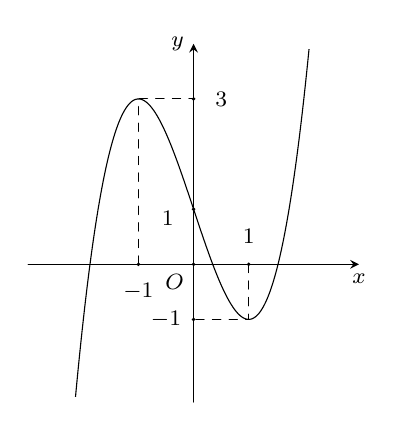
\begin{tikzpicture}[scale=0.7,>=stealth, font=\footnotesize, line join=round, line cap=round]
			\def\a{1} \def\b{0} \def\c{-3} \def\d{1} % Hệ số
			\def\xmin{-3} \def\xmax{3}
			\def\ymin{-2.5} \def\ymax{4}
			%\draw[color=gray!50,dashed] (\xmin,\ymin) grid (\xmax,\ymax);
			\draw[->] (\xmin,0)--(\xmax,0) node [below]{$x$};
			\draw[->] (0,\ymin)--(0,\ymax) node [left]{$y$};
			\node at (0,0) [below left]{$O$};
			\clip (\xmin+0.1,\ymin+0.1) rectangle (\xmax-0.5,\ymax-0.1);
			\draw[smooth,samples=300] plot(\x,{\a*(\x)^3+\b*(\x)^2+\c*(\x)+\d});
			\fill (-1,0)node[shift={(270:0.35)}]{$-1$} circle(1pt);
			\fill (1,0)node[shift={(90:0.35)}]{$1$} circle(1pt);
\fill (0,3)node[shift={(0:0.35)}]{$3$} circle(1pt);
			\fill (0,-1)node[shift={(180:0.35)}]{$-1$} circle(1pt);
			\fill (0,1)node[shift={(200:0.35)}]{$1$} circle(1pt);
	\fill (0,0) circle(1pt);
\draw[dashed] (-1,0)--(-1,3)--(0,3);
\draw[dashed] (1,0)--(1,-1)--(0,-1);
		\end{tikzpicture}
	}

	\loigiai
	{Dựa vào đồ thị suy ra hàm số thỏa mãn có dạng $y=ax^3+bx^2+cx+d$, hệ số $a>0,d>0$.\\
		Vậy hàm số thỏa mãn là $y=x^3-3x+1$.}
\end{ex}

\begin{ex}%[Đề thi GHK1-THPT Nguyễn Duy Hiệu - Quảng Nam, năm 2020]%[Nguyễn Trung Kiên, dự án 12-EX-3-2021]%[2D1Y5-5]
    Cho hàm số $f(x)$ xác định trên $\mathbb{R}$ và có đồ thị hàm số $f'(x)$ là đường cong trong hình sau. Mệnh đề nào dưới đây đúng?
    \immini
    {\choice
        {Hàm số $f(x)$ nghịch biến trên khoảng$(-1;1)$}
        {Hàm số $f(x)$ đồng biến trên khoảng $(1;2)$}
        {Hàm số $f(x)$ đồng biến trên khoảng $(-2;1)$}
        {\True Hàm số $f(x)$ nghịch biến trên khoảng $(0;2)$}}
    {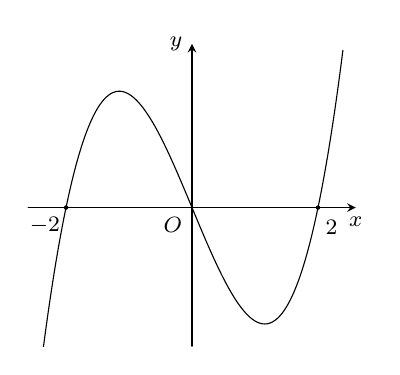
\begin{tikzpicture}[scale=0.8, font=\footnotesize,line join=round, line cap=round, >=stealth]
            \draw[->] (-2.6,0)--(0,0)node[below left]{$O$}--(2.6,0) node[below]{$x$};
            \draw[->] (0,-2.2)--(0,2.6)node[left]{$y$};
            \clip (-2.6,-2.2) rectangle (2.5,2.5);
            \draw[smooth,samples=150,domain=-2.5:2.5] plot (\x,{0.6*(\x)^3-2.4*(\x)});
            \fill (-2,0)node[shift={(220:0.35)}]{$-2$} circle(1pt);
            \fill (2,0)node[shift={(-55:0.3)}]{$2$} circle(1pt);
    \end{tikzpicture}}
    \loigiai
    {Từ đồ thị hàm số $y=f'(x)$ ta có $f'(x)<0,\, \forall x\in (0;2)$ nên hàm số $y=f(x)$ nghịch biến trên khoảng $(0;2)$.}
\end{ex}

\begin{ex}%[Đề thi GHK1-THPT Nguyễn Duy Hiệu - Quảng Nam, năm 2020]%[Nguyễn Trung Kiên, dự án 12-EX-3-2021]%[2D1Y5-8]
    Cho hàm số $y=f(x)=ax^3+bx^2+cx+d\,(a\neq 0)$. Khẳng định nào sau đây đúng?
    \choice
    {Đồ thị hàm số luôn có tiệm cận}
    {Hàm số luôn có cực trị}
    {\True Đồ thị hàm số luôn cắt trục hoành}
    {$\lim\limits_{x\to \pm \infty}f(x)=\pm \infty$}
    \loigiai
    {Ta có $f(x)$ là hàm số liên tục trên $\mathbb{R}$.\\
    Nếu $a>0$ thì $\lim\limits_{x \to -\infty}f(x)=-\infty$; $\lim\limits_{x \to +\infty}f(x)=+\infty$.\\
    Nếu $a<0$ thì $\lim\limits_{x \to -\infty}f(x)=+\infty$; $\lim\limits_{x \to +\infty}f(x)=-\infty$.\\
    Do đó đồ thị hàm số luôn cắt trục hoành.}
\end{ex}

\begin{ex}%[Đề thi GHK1-THPT Nguyễn Duy Hiệu - Quảng Nam, năm 2020]%[Nguyễn Trung Kiên, dự án 12-EX-3-2021]%[2H1Y1-3]
    Mặt phẳng $\left(AB'C'\right)$ chia khối lăng trụ $ABC.A'B'C'$ thành
    \choice
    {Hai khối chóp tứ giác}
    {Hai khối chóp tam giác}
    {Một khối chóp tam giác và một khối chóp ngũ giác}
    {\True Một khối chóp tam giác và một khối chóp tứ giác}
    \loigiai
    {\immini
        {Mặt phẳng $\left(AB'C'\right)$ chia khối lăng trụ $ABC.A'B'C'$ thành khối chóp tam giác $A.A'B'C'$ và khối chóp tứ giác $A.BCC'B'$.}
        {\begin{tikzpicture}[scale=1, font=\footnotesize,line join=round, line cap=round, >=stealth]
                \def \h{3.5}
                \path (0,0) coordinate(A)
                (0:4)coordinate(C)
                (1.5,-1.2) coordinate(B);
                \foreach \i in {A,B,C} {\path ($(\i)+(-0.5,\h)$) coordinate(\i');}
                \draw (A)--(B)--(C)--(C')--(A')--(B')--(C') (A)--(A') (B)--(B') (A)--(B');
                \draw[dashed] (A)--(C) (A)--(C');
                \foreach \diem/\pos in {A/180, B/-90, C/0, A'/180, B'/90, C'/0} \fill (\diem) node[shift={(\pos:0.3)}] {$\diem$} circle(1pt);
    \end{tikzpicture}}}
\end{ex}

\begin{ex}%[GHK I, THPT Nguyên Duy Hiệu, Quang Nam, 2021]%[Huỳnh Xuân Tín, 12-EX-2-2021]%[2H1Y2-2]
Số cạnh của một hình mười hai mặt đều là
	\choice
	{\True $30$}
	{$12$}
	{$24$}
	{$20$}
	\loigiai
	{Số cạnh của một hình mười hai mặt đều là $30$.
		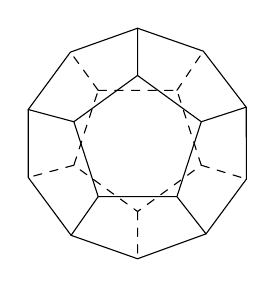
\begin{tikzpicture}[font=\footnotesize, line join=round, line cap=round, >=stealth]
		%	\begin{scope}
				\draw[black](0,0)coordinate(a1)--++(0:1)coordinate(a2)--++(72:1)coordinate(a3)--++(144:1)coordinate(a4)--++(216:1)coordinate(a5)--(0,0);
				\draw[dashed] (0,1.35)coordinate(b1)--++(0:1)coordinate(b2)--++(-72:1)coordinate(b3)--++(-144:1)coordinate(b4)--++(-216:1)coordinate(b5)--(0,1.35);
				\draw[black] (a4)--++(90:0.6)coordinate(c1)(a1)--++(235:0.6)coordinate(c2)(a2)--++(-52:0.6)coordinate(c3)(a3)--++(18:0.6)coordinate(c4)(a5)--++(165:0.6)coordinate(c5);
				\draw[dashed] (b5)--++(195:0.6)coordinate(c6)(b4)--++(-90:0.6)coordinate(c7)(b3)--++(-17:0.6)coordinate(c8)(b2)--++(56:0.6)coordinate(c9)(b1)--++(126:0.6)coordinate(c10);
				\draw[black] (c1)--(c10)--(c5)--(c6)--(c2)--(c7)--(c3)--(c8)--(c4)--(c9)--(c1);
				\tkzDrawPoints[fill=black](a1,a2,a3,a4,a5,b1,b2,b3,b4,b5,c1,c2,c3,c4,c5,c6,c7,c8,c9,c10)
		%	\end{scope}
	\end{tikzpicture}}
\end{ex}

\begin{ex}%[GHK I, THPT Nguyên Duy Hiệu, Quang Nam, 2021]%[Huỳnh Xuân Tín, 12-EX-2-2021]%[2H1Y2-3]
Hình chóp tứ giác đều có bao nhiêu mặt phẳng đối xứng?
	\choice
	{$2$}
	{\True $4$}
	{$8$}
	{$6$}
	\loigiai
	{Hình chóp tứ giác đều có $4$ mặt phẳng đối xứng là
		\begin{center}
			\begin{minipage}{0.2\textwidth}
				\begin{tikzpicture}[scale=0.8, font=\footnotesize, line join=round, line cap=round, >=stealth]
					\tkzDefPoints{0/0/D,3.5/0/C,1.2/1/A}
					\coordinate (B) at ($(A)+(C)-(D)$);
					\tkzInterLL(A,C)(B,D)    \tkzGetPoint{O}
					\coordinate (S) at ($(O)+(0,3)$);
					\coordinate (M) at ($0.5*(A)+0.5*(B)$);
					\coordinate (N) at ($0.5*(C)+0.5*(B)$);
					\coordinate (P) at ($0.5*(C)+0.5*(D)$);
					\coordinate (Q) at ($0.5*(A)+0.5*(D)$);
					\tkzDrawPolygon[white,pattern=dots](S,M,P)
					\tkzDrawPolygon(S,B,C,D)
					\tkzDrawSegments(S,C S,P)
					\tkzDrawSegments[dashed](M,P S,M A,S A,B A,D A,C B,D S,O)
					\tkzDrawPoints[fill=black](M,P,D,C,A,B,O,S)
				\end{tikzpicture}
				\newline\textbf{\centering \scriptsize Hình $1$.}
			\end{minipage}
			\begin{minipage}{0.2\textwidth}
				\begin{tikzpicture}[scale=0.8, font=\footnotesize, line join=round, line cap=round, >=stealth]
					\tkzDefPoints{0/0/D,3.5/0/C,1.2/1/A}
					\coordinate (B) at ($(A)+(C)-(D)$);
					\tkzInterLL(A,C)(B,D)    \tkzGetPoint{O}
					\coordinate (S) at ($(O)+(0,3)$);
					\coordinate (M) at ($0.5*(A)+0.5*(B)$);
					\coordinate (N) at ($0.5*(C)+0.5*(B)$);
					\coordinate (P) at ($0.5*(C)+0.5*(D)$);
					\coordinate (Q) at ($0.5*(A)+0.5*(D)$);
					\tkzDrawPolygon[white,pattern=dots](S,A,C)
					\tkzDrawPolygon(S,B,C,D)
					\tkzDrawSegments(S,C)
					\tkzDrawSegments[dashed](A,S A,B A,D A,C B,D S,O)
					\tkzDrawPoints[fill=black](D,C,A,B,O,S)
				\end{tikzpicture}
				\newline\textbf{\centering \scriptsize Hình $2$.}
			\end{minipage}
			\begin{minipage}{0.2\textwidth}
				\begin{tikzpicture}[scale=0.8, font=\footnotesize, line join=round, line cap=round, >=stealth]
					\tkzDefPoints{0/0/D,3.5/0/C,1.2/1/A}
					\coordinate (B) at ($(A)+(C)-(D)$);
					\tkzInterLL(A,C)(B,D)    \tkzGetPoint{O}
					\coordinate (S) at ($(O)+(0,3)$);
					\coordinate (M) at ($0.5*(A)+0.5*(B)$);
					\coordinate (N) at ($0.5*(C)+0.5*(B)$);
					\coordinate (P) at ($0.5*(C)+0.5*(D)$);
					\coordinate (Q) at ($0.5*(A)+0.5*(D)$);
					\tkzDrawPolygon[white,pattern=dots](S,N,Q)
					\tkzDrawPolygon(S,B,C,D)
					\tkzDrawSegments(S,N S,C)
					\tkzDrawSegments[dashed](S,Q N,Q A,S A,B A,D A,C B,D S,O)
					\tkzDrawPoints[fill=black](N,Q,D,C,A,B,O,S)
				\end{tikzpicture}
				\newline\textbf{\centering \scriptsize Hình $3$.}
			\end{minipage}
			\begin{minipage}{0.2\textwidth}
				\begin{tikzpicture}[scale=0.8, font=\footnotesize, line join=round, line cap=round, >=stealth]
					\tkzDefPoints{0/0/D,3.5/0/C,1.2/1/A}
					\coordinate (B) at ($(A)+(C)-(D)$);
					\tkzInterLL(A,C)(B,D)    \tkzGetPoint{O}
					\coordinate (S) at ($(O)+(0,3)$);
					\coordinate (M) at ($0.5*(A)+0.5*(B)$);
					\coordinate (N) at ($0.5*(C)+0.5*(B)$);
					\coordinate (P) at ($0.5*(C)+0.5*(D)$);
					\coordinate (Q) at ($0.5*(A)+0.5*(D)$);
					\tkzDrawPolygon[white,pattern=dots](S,B,D)
					\tkzDrawPolygon(S,B,C,D)
					\tkzDrawSegments(S,C)
					\tkzDrawSegments[dashed](A,S A,B A,D A,C B,D S,O)
					\tkzDrawPoints[fill=black](D,C,A,B,O,S)
				\end{tikzpicture}
				\newline\textbf{\centering \scriptsize Hình $4$.}
			\end{minipage}
	\end{center}}
\end{ex}

\begin{ex}%[GHK I, THPT Nguyên Duy Hiệu, Quang Nam, 2021]%[Huỳnh Xuân Tín, 12-EX-2-2021]%[2H1Y3-2]
	Một khối hộp chữ nhật có ba kích thước là $a$, $2a$ và $3a$. Thể tích của khối hộp chữ nhật đó	bằng
	\choice
	{$a^3$}
	{$2a^3$}
	{$6a^3$}
	{\True $3a^3$}
	\loigiai
	{Thể tích của khối hộp chữ nhật có ba kích thước là $a$, $2a$ và $3a$ đó	bằng $a\cdot 2a\cdot 3a=6 a^3$.}
\end{ex}

\begin{ex}%[GHK I, THPT Nguyên Duy Hiệu, Quang Nam, 2021]%[Huỳnh Xuân Tín, 12-EX-2-2021]%[2H1Y3-2]
Thể tích của khối hộp có diện tích đáy bằng $S$ và có chiều cao bằng $h$ là
	\choice
	{$\dfrac{Sh}{6}$}
	{$\dfrac{Sh}{2}$}
	{$\dfrac{Sh}{3}$}
	{\True $Sh$}
		\loigiai
	{Thể tích của khối hộp có diện tích đáy bằng $S$ và có chiều cao bằng $h$ là	$V=S\cdot h$.}
\end{ex}

\begin{ex}%[Đề thi GHK1-THPT Nguyễn Duy Hiệu - Quảng Nam, năm 2020]%[Nguyễn Trung Kiên, dự án 12-EX-3-2021]%[2H1Y3-4]
    Khối chóp có thể tích bằng $V$, diện tích đáy bằng $S$ có chiều cao bằng
    \choice
    {\True $\dfrac{3V}{S}$}
    {$\dfrac{V}{3S}$}
    {$\dfrac{V}{S}$}
    {$\dfrac{3S}{V}$}
    \loigiai
    {Ta có $V=\dfrac{1}{3}Sh\Rightarrow h=\dfrac{3V}{S}$.}
\end{ex}

\begin{ex}%[GHK I, THPT Nguyên Duy Hiệu, Quang Nam, 2021]%[Huỳnh Xuân Tín, 12-EX-2-2021]%[2H1Y3-4]
Cho hình chóp $S.ABCD$ có diện tích đáy $ABCD$ bằng $2$ và thể tích khối chóp $S.ABCD$ bằng $4$. Khi đó khoảng cách từ $S$ tới mặt phẳng đáy bằng bao nhiêu?
	\choice
	{$9$}
	{$2$}
	{$6$}
	{\True $3$}
	\loigiai
	{Ta có $V_{S.ABCD}=\dfrac{1}{3}\cdot \mathrm{d}[S,(ABCD)] \cdot S_{ABCD}\Leftrightarrow 4=\dfrac{1}{3}\cdot \mathrm{d}[S,(ABCD)] \cdot 2\Leftrightarrow \mathrm{d}[S,(ABCD)]=6$.}
\end{ex}

\begin{ex}%[Đề thi GHK1-THPT Nguyễn Duy Hiệu - Quảng Nam, năm 2020]%[Nguyễn Trung Kiên, dự án 12-EX-3-2021]%[2D1B1-1]
    Cho hàm số $y=-x^3+3x^2-3x+2$. Khẳng định nào sau đây là khẳng định đúng?
    \choice
    {\True Hàm số luôn nghịch biến trên $\mathbb{R}$}
    {Hàm số đồng biến trên khoảng $(-\infty ;1)$ và nghịch biến trên khoảng $(1;+\infty)$}
    {Hàm số luôn đồng biến trên $\mathbb{R}$}
    {Hàm số đồng biến trên các khoảng $(-\infty ;1)$ và $(1;+\infty)$}
    \loigiai
    {Hàm số $y=-x^3+3x^2-3x+2$ xác định trên tập $\mathbb{R}$. Ta có
    \[y'=-3x^2+6x-3=-3(x-1)^2\leq 0,\, \forall x\in \mathbb{R}.\]
    Vậy hàm số nghịch biến trên $\mathbb{R}$.}
\end{ex}

\begin{ex}%[Đề thi GHK1-THPT Nguyễn Duy Hiệu - Quảng Nam, năm 2020]%[Nguyễn Trung Kiên, dự án 12-EX-3-2021]%[2D1B1-1]
    Cho hàm số $y=\dfrac{x+1}{1-x}$. Khẳng định nào sao đây là khẳng định đúng?
    \choice
    {\True Hàm số đồng biến trên các khoảng $(-\infty ;1 )$ và $(1;+\infty)$}
    {Hàm số nghịch biến trên các khoảng $(-\infty ;1)$ và $(1;+\infty)$}
    {Hàm số đồng biến trên khoảng $(-\infty ;1)\cup (1;+\infty)$}
    {Hàm số nghịch biến trên khoảng $(-\infty ;1)\cup (1;+\infty)$}
    \loigiai
    {Tập xác định $\mathscr{D}=\mathbb{R}\setminus\{1\}$.\\
    Ta có $y'=\dfrac{2}{(x-1)^2}>0,\,\forall x\neq 1$ nên hàm số đồng biến trên các khoảng $(-\infty;1)$ và $(1;+\infty)$.}
\end{ex}

\begin{ex}%[GHK I, THPT Nguyên Duy Hiệu, Quang Nam, 2021]%[Huỳnh Xuân Tín, 12-EX-2-2021]%[2D1B1-3]
Cho hàm số sau $y=-\dfrac{1}{3} x^3-m x^2+(2 m-3) x-m+2$. Tổng các giá trị nguyên của tham số $m$ để	hàm số luôn nghịch biến trên $\mathbb{R}$?
	\choice
	{$-3$}
	{\True $-5$}
	{$0$}
	{$-2$}
	\loigiai
	{Ta có $y'=-x^2-2mx+2m-3$.\\
	Để hàm số luôn nghịch biến trên $\mathbb{R}$ khi và chỉ khi $y'\le 0, \forall x\in \mathbb{R}$. Điều này tương đương với $\Delta'=m^2+2m-3\le 0\Leftrightarrow -3\le m\le 1$.\\
Với $m$ nguyên nên $m\in \{-3;-2;-1;0;1\}$. Khi đó tổng các giá trị nguyên của tham số $m$ để	hàm số luôn nghịch biến trên $\mathbb{R}$ là $-3-2-1+0+1=-5$.}
\end{ex}

\begin{ex}%[Đề thi GHK1-THPT Nguyễn Duy Hiệu - Quảng Nam, năm 2020]%[Nguyễn Trung Kiên, dự án 12-EX-3-2021]%[2D1B2-1]
    Giá trị cực đại của hàm số $y=x^3-3x^2-9x-3$ là
    \choice
    {$3$}
    {$-1$}
    {$-30$}
    {\True $2$}
    \loigiai
    {Hàm số $y=x^3-3x^2-9x-3$ có tập xác định $\mathscr{D}=\mathbb{R}$, $y'=3x^2-6x-9$.\\
        Ta có $y'=0\Leftrightarrow \hoac{&x=-1\\&x=3}$, do đó ta có bảng biến thiên của hàm số
        \begin{center}
            
\begin{tikzpicture}[scale=1, font=\footnotesize,line join=round, line cap=round, >=stealth]
                \tkzTabInit[nocadre=false,lgt=1.2,espcl=3]
                {$x$ /0.6,$y'$ /0.6,$y$ /2}
                {$-\infty$,$-1$,$3$,$+\infty$}
                \tkzTabLine{,+,$0$,-,$0$,+,}
                \tkzTabVar{-/$-\infty$, +/$2$,-/$-30$,+/$+\infty$}
            \end{tikzpicture}
        \end{center}
        Vậy ta thấy hàm số có giá trị cực đại là $y_{\text{CĐ}}=y(-1)=2$.}
\end{ex}

\begin{ex}%[Đề thi GHK1-THPT Nguyễn Duy Hiệu - Quảng Nam, năm 2020]%[Nguyễn Trung Kiên, dự án 12-EX-3-2021]%[2D1B3-1]
    Cho hàm số $y=-x^3+3x+5$. Chọn phương án đúng trong các phương án sau.
    \choice
    {$\max\limits_{[-1;1]}=3$}
    {\True $\min\limits_{[0;2]}=3$}
    {$\max\limits_{[0;2]}=5$}
    {$\min\limits_{[-1;1]}=7$}
    \loigiai
    {Xét hàm số $y=-x^3+3x+5$.
    Ta có $y'=-3x^2+3$, $y'=0\Leftrightarrow \hoac{&x=-1\\&x=1.}$\\
    Mà $y(-1)=3$, $y(1)=7$, $y(0)=5$, $y(2)=3$ nên
    \[\max\limits_{[-1;1]}=7;\, \min\limits_{[-1;1]}=3;\, \max\limits_{[0;2]}=7;\, \min\limits_{[0;2]}=3.\]}
\end{ex}

\begin{ex}%[GHK I, THPT Nguyên Duy Hiệu, Quang Nam, 2021]%[Huỳnh Xuân Tín, 12-EX-2-2021]%[2D1B2-1]
    Hàm số nào sau đây không có cực trị?
    \choice
    {$y=x^3+3x^2$}
    {$y=x^4-3x^2+2$}
    {\True $y=x^3$}
    {$y=x^3-x$}
    \loigiai
    {Ta có
        \begin{itemize}
            \item Hàm số $y=x^3+3x^2$ có $y'=3x^2+6x=0\Leftrightarrow\heva{&x=0\\&x=-2}$ nên hàm số có hai cực trị (vì $y'$ là bậc $2$).
            \item  Hàm số $y=x^4-3x^2+2$ có $y'=4x^3-6x=0\Leftrightarrow\heva{&x=0\\&x=\pm \dfrac{3}{2}}$ nên hàm số có ba điểm cực trị nên hàm số có cực trị (vì $y'$ là bậc $3$).
            \item Hàm số $y=x^3$ có $y'=3x^2\ge 0$, $\forall x\in \mathbb{R}$ nên hàm số không có cực trị.
            \item Hàm số $y=x^3-x$ có $y'=3x^2-1=0\Leftrightarrow x=\pm \sqrt{\dfrac{1}{3}}$ nên hàm số có hai cực trị (vì $y'$ là bậc $2$).
    \end{itemize}}
\end{ex}

\begin{ex}%[GHK I, THPT Nguyên Duy Hiệu, Quang Nam, 2021]%[Huỳnh Xuân Tín, 12-EX-2-2021]%[2D1B3-1]
	Tìm các giá trị của tham số $m$ để giá trị nhỏ nhất của hàm số $f(x)=\dfrac{x-m^2+m}{x+1}$ trên đoạn $[0; 1]$ bằng $-2$.
	\choice
	{$m=1;\,m=-2$}
	{$m=-1;\,m=-2$}
	{$m=1;\,m=2$}
	{\True $m=-1;\,m=2$}
	\loigiai
	{Ta có $f'(x)=\dfrac{m^2-m+1}{(x+1)^2}>0, \forall x\in [0;1]$. Khi đó hàm số đã cho đồng biến trên $[0;1]$. Do đó
		\[\min\limits_{x\in[0;1]} f(x)=f(0)=-m^2+m=-2\Leftrightarrow \hoac{&m=-1\\&m=2.}\]
Vậy giá trị của $m$ cần tìm là $-1;2$.	}
\end{ex}

\begin{ex}%[Đề thi GHK1-THPT Nguyễn Duy Hiệu - Quảng Nam, năm 2020]%[Nguyễn Trung Kiên, dự án 12-EX-3-2021]%[2D1B3-2]
    Tìm mệnh đề đúng
    \choice
    {\True Trên khoảng $(0; +\infty)$ thì hàm số $y=-x^3+3x+1$ có giá trị lớn nhất bằng $3$}
    {Trên khoảng $(0; +\infty)$ thì hàm số $y=-x^3+3x+1$ có giá trị nhỏ nhất bằng $-1$}
    {Trên khoảng $(0; +\infty)$ thì hàm số $y=-x^3+3x+1$ có giá trị lớn nhất bằng $1$}
    {Trên khoảng $(0; +\infty)$ thì hàm số $y=-x^3+3x+1$ có giá trị nhỏ nhất bằng $3$}
    \loigiai
    {Xét hàm số $y=-x^3+3x+1$ trên khoảng $(0;+\infty)$.\\
        Ta có $y'=-3x^2+3$, $y'=0\Leftrightarrow \hoac{&x=-1 \notin (0;+\infty)\\&x=1\in (0;+\infty).}$\\
        Bảng biến thiên
        \begin{center}
            
\begin{tikzpicture}[scale=1, font=\footnotesize,line join=round, line cap=round, >=stealth]
                \tkzTabInit[nocadre=false,lgt=1.2,espcl=3.5]
                {$x$ /0.6,$y'$ /0.6,$y$ /2}
                {$0$,$1$,$+\infty$}
                \tkzTabLine{,+,$0$,-,}
                \tkzTabVar{-/$1$, +/$3$,-/$-\infty$}
            \end{tikzpicture}
        \end{center}
        Dựa vào bảng biến thiêu suy ra $\max\limits_{(0;+\infty)}y=3$ khi $x=1$.}
\end{ex}

\begin{ex}%[Đề thi GHK1-THPT Nguyễn Duy Hiệu - Quảng Nam, năm 2020]%[Nguyễn Trung Kiên, dự án 12-EX-3-2021]%[2D1B3-2]
    Cho hàm số $y=3\sin{x}-4\sin^3{x}$. Giá trị lớn nhất của hàm số trên khoảng $\left(-\dfrac{\pi}{2};\dfrac{\pi}{2} \right)$ bằng
    \choice
    {$3$}
    {\True $1$}
    {$-1$}
    {$7$}
    \loigiai
    {\begin{itemize}
            \item [$\bullet$] \textbf{Cách 1:} Đặt $\sin{x}=t$, với $x\in \left(-\dfrac{\pi}{2};\dfrac{\pi}{2}\right)$ thì $t\in (-1;1)$ ta được hàm số $f(t)=3t-4t^3$ xác định và liên tục trên $(-1;1)$.\\
            Ta có $f'(t)=3-12t^2$, $f'(t)=0\Leftrightarrow t=\pm \dfrac{1}{2}\in (-1;1)$. Suy ra bảng biến thiên
            \begin{center}
                
\begin{tikzpicture}
                    \tkzTabInit[nocadre=false,lgt=1.2,espcl=3]
                    {$x$ /0.7,$y'$ /0.7,$y$ /2}
                    {$-1$,$-\tfrac{1}{2}$,$\tfrac{1}{2}$,$1$}
                    \tkzTabLine{,-,$0$,+,$0$,-,}
                    \tkzTabVar{+/$1$, -/$-1$,+/$1$,-/$-1$}
                \end{tikzpicture}
            \end{center}
        Vậy $\max\limits_{ \left(-\tfrac{\pi}{2};\tfrac{\pi}{2}\right)}y =\max\limits_{(-1;1)}f(t)=1$.
            \item [$\bullet$] \textbf{Cách 2:} Với $x\in \left(-\dfrac{\pi}{2};\dfrac{\pi}{2}\right)\Rightarrow 3x\in \left(-\dfrac{3\pi}{2};\dfrac{3\pi}{2}\right)$. Do đó
            \[y=3\sin{x}-4\sin^3{x}=\sin3x\leq 1\Rightarrow \max\limits_{ \left(-\tfrac{\pi}{2};\tfrac{\pi}{2}\right)}y=1.\]
    \end{itemize}}
\end{ex}

\begin{ex}%[GHK I, THPT Nguyên Duy Hiệu, Quang Nam, 2021]%[Huỳnh Xuân Tín, 12-EX-2-2021]%[2D1B4-1]
	Cho hàm số $y=\dfrac{2x+1}{x-1}$. Đồ thị hàm số có tâm đối xứng là điểm
	\choice
	{$(2;1)$}
	{\True $(1;2)$}
	{$(-1;1)$}
	{$(1;-1)$}
	\loigiai
	{Đồ thị hàm số $y=\dfrac{2x+1}{x-1}$ có tâm đối xứng là giao điểm của hai tiệm cận.\\
	Hàm số có tiệm cận đứng là $x=1$, tiệm cận ngang là $y=2$. Do đó tâm đối xứng của đồ thị là $I(1;2)$.}
\end{ex}

\begin{ex}%[Đề thi GHK1-THPT Nguyễn Duy Hiệu - Quảng Nam, năm 2020]%[Nguyễn Trung Kiên, dự án 12-EX-3-2021]%[2D1B5-3]
    Cho hàm số $y=x^3-3x^2+1$. Đồ thị hàm số cắt đường thẳng $y=m$ tại $3$ điểm phân biệt khi
    \choice
    {$m<-3$}
    {\True $-3<m<1$}
    {$-3\leq m\leq 1$}
    {$m>1$}
    \loigiai
    {Hàm số $y=x^3-3x^2+1$ có tập xác định $\mathscr{D}=\mathbb{R}$, $y'=3x^2-6x$.\\
    Ta có $y'=0\Leftrightarrow \hoac{&x=0\\&x=2}$. Vì vậy ta có bảng biến thiên
    \begin{center}
        
\begin{tikzpicture}
            \tkzTabInit[nocadre=false,lgt=1.2,espcl=3]
            {$x$ /0.6,$y'$ /0.6,$y$ /2}
            {$-\infty$,$0$,$2$,$+\infty$}
            \tkzTabLine{,+,$0$,-,$0$,+,}
            \tkzTabVar{-/$-\infty$, +/$1$,-/$-3$,+/$+\infty$}
        \end{tikzpicture}
    \end{center}
    Dựa vào bảng biến thiên ta thấy đường thẳng $y=m$ cắt đồ thị hàm số tại ba điểm phân biệt khi và chỉ khi $-3<m<1$.}
\end{ex}

\begin{ex}%[Đề thi GHK1-THPT Nguyễn Duy Hiệu - Quảng Nam, năm 2020]%[Nguyễn Trung Kiên, dự án 12-EX-3-2021]%[2D1B5-3]
    Cho hàm số $y=x^3+4x$. Số giao điểm của đồ thị hàm số và trục $Ox$ bằng
    \choice
    {$2$}
    {\True $1$}
    {$3$}
    {$4$}
    \loigiai
    {Xét phương trình hoành độ giao điểm của đồ thị hàm số và trục $Ox$, ta có
    \[x^3+4x=0 \Leftrightarrow x\left(x^2+4\right)=0 \Leftrightarrow x=0.\]
    Vậy đồ thị hàm số và trục $Ox$ có đúng một điểm chung.}
\end{ex}

\begin{ex}%[Đề thi GHK1-THPT Nguyễn Duy Hiệu - Quảng Nam, năm 2020]%[Nguyễn Trung Kiên, dự án 12-EX-3-2021]%[2D1B5-7]
    Trên đồ thị $(H)$ của hàm số $y=\dfrac{3-x}{2x-1}$. Có bao nhiêu điểm có tọa độ nguyên?
    \choice
    {$3$}
    {$1$}
    {\True $4$}
    {$2$}
    \loigiai
    {Tập xác định $\mathscr{D}=\mathbb{R}\setminus\left\{\dfrac{1}{2}\right\}$. Hàm số $y=\dfrac{3-x}{2x-1}$ đơn điệu trên các khoảng xác định của nó.\\
    Ta có $\lim\limits_{x\to \pm \infty}y=-\dfrac{1}{2}$, do đó
    $-1<y<0 \Leftrightarrow -1<\dfrac{3-x}{2x-1}<0 \Leftrightarrow \hoac{&x<-2\\&x>3.}$\\
    Mà $y(-2)=-1$, $y(-1)=-\dfrac{4}{3}$, $y(0)=-3$, $y(1)=2$, $y(2)=\dfrac{1}{3}$, $y(3)=0$ nên đồ thị hàm số có $4$ điểm có tọa độ nguyên là $(-2;-1)$, $(0;-3)$, $(1;2)$ và $(3;0)$.}
\end{ex}

\begin{ex}%[Đề thi GHK1-THPT Nguyễn Duy Hiệu - Quảng Nam, năm 2020]%[Nguyễn Trung Kiên, dự án 12-EX-3-2021]%[2H1B3-2]
    Cho khối lăng trụ đứng tam giác $ABC.A'B'C'$ có đáy là một tam giác vuông tại $A$. Cho $AC=AB=2a$, góc giữa $AC'$ và mặt phẳng $(ABC)$ bằng $30^\circ$. Tính thể tích khối lăng trụ $ABC.A'B'C'$.
    \choice
    {$\dfrac{2a^3\sqrt{3}}{3}$}
    {$\dfrac{a^3\sqrt{3}}{3}$}
    {$\dfrac{a^3\sqrt{3}}{2}$}
    {\True $\dfrac{4a^3\sqrt{3}}{3}$}
    \loigiai
    {\immini
        {Tam giác $ABC$ vuông cân tại $A$ nên
        \[S=S_{ABC}=\dfrac{1}{2}\cdot AB\cdot AC=2a^2.\]
        Lại có $ABC.A'B'C'$ là lăng trụ đứng nên $\left(AC',(ABC)\right)=\widehat{CAC'}$. Từ đó ta có
        \[h=CC'=AC\cdot \tan\widehat{CAC'}=2a\tan 30^\circ = \dfrac{2a\sqrt{3}}{3}.\]
        Vậy thể tích khối lăng trụ $ABC.A'B'C'$ là
        \[V_{ABC.A'B'C'}=Sh=2a^2\cdot \dfrac{2a\sqrt{3}}{3} = \dfrac{4a^3\sqrt{3}}{3}.\]}
        {\begin{tikzpicture}[scale=1, font=\footnotesize,line join=round, line cap=round, >=stealth]
                \def \h{3.5}
                \path (0,0) coordinate(A)
                (0:4)coordinate(C)
                (1.5,-1.2) coordinate(B);
                \foreach \i in {A,B,C} {\path ($(\i)+(0,\h)$) coordinate(\i');}
                \draw (A)--(B)--(C)--(C')--(A')--(B')--(C') (A)--(A') (B)--(B');
                \draw[dashed] (A)--(C) (A)--(C');
                \foreach \diem/\pos in {A/180, B/-90, C/0, A'/180, B'/90, C'/0} \fill (\diem) node[shift={(\pos:0.3)}] {$\diem$} circle(1pt);
                \tkzMarkRightAngles[size=0.2](C',C,A B,A,C)
                \node at (A)[shift={(20:0.45)},rotate=15]{\scriptsize $30^\circ$};
                \tkzMarkAngles[size=0.7](C,A,C')
    \end{tikzpicture}}}
\end{ex}

\begin{ex}%[GHK I, THPT Nguyên Duy Hiệu, Quang Nam, 2021]%[Huỳnh Xuân Tín, 12-EX-2-2021]%[2H1B3-2]
	Cho hình chóp $S.ABC$ có $SA\perp (ABC)$, đáy  là tam giác đều cạnh $2a$, $SB=2a\sqrt{2}$. Thể tích
	của khối chóp $S.ABC$ bằng
	\choice
	{$\dfrac{a^3\sqrt{6}}{3}$}
	{\True $\dfrac{2a^3\sqrt{3}}{3}$}
	{$2a^3\sqrt{3}$}
	{$\dfrac{2a^3\sqrt{6}}{3}$}
	\loigiai
	{\immini{Xét $\triangle SAB$ vuông tại $A$ ta có $SA=\sqrt{SB^2-AB^2}=2a$.\\
		$\triangle ABC$ đều có cạnh $2a$ nên có diện tích $\dfrac{(2a)^2\sqrt{3}}{4}=a^2\sqrt{3}$.\\
	Vậy thể tích khối chóp $S.ABC$ là
\[V=\dfrac{1}{3}\cdot SA\cdot S_{ABC}=\dfrac{1}{3}\cdot2a\cdot a^2\sqrt{3}=\dfrac{2a^3\sqrt{3}}{3}. \]}{\begin{tikzpicture}[scale=1,>=stealth, font=\footnotesize, line join=round, line cap=round]
				\tkzDefPoints{0/0/A,1.2/-1.5/B,4/0/C}
				\coordinate (S) at ($(A)+(0,3)$);
				\tkzDrawPolygon(S,A,B,C)
				\tkzDrawSegments(S,B)
				\tkzDrawSegments[dashed](A,C)
				\tkzDrawPoints[fill=black](A,B,C,S)
				\tkzMarkRightAngles[size=0.16](S,A,B S,A,C)
				\tkzLabelPoints[above](S)
				\tkzLabelPoints[below](B)
				\tkzLabelPoints[left](A)
				\tkzLabelPoints[right](C)
	\end{tikzpicture}}}
\end{ex}

\begin{ex}%[Đề thi GHK1-THPT Nguyễn Duy Hiệu - Quảng Nam, năm 2020]%[Nguyễn Trung Kiên, dự án 12-EX-3-2021]%[2H1B3-3]
    Cho hình chóp $S.ABC$. Gọi $G$ là trọng tâm của tam giác $SBC$, mặt phẳng $(\alpha)$ đi qua $AG$ và song song với $BC$ chia khối chóp thành hai phần. Gọi $V_1$ là thể tích của khối đa diện chứa đỉnh $S$ và $V_2$ là thể tích của khối đa diện không chứa đỉnh $S$. Tính tỉ số $\dfrac{V_1}{V_2}$.
    \choice
    {\True $\dfrac{4}{5}$}
    {$\dfrac{5}{9}$}
    {$\dfrac{1}{3}$}
    {$\dfrac{4}{9}$}
    \loigiai
    {\immini
        {Gọi $M$ là trung điểm của $BC$. Mặt phẳng $(\alpha)$ và mặt phẳng $(SBC)$ có $G$ là một điểm chung và $(\alpha)\parallel BC$ nên giao tuyến của $(\alpha)$ và $(SBC)$ là đường thẳng đi qua $G$, song song với $BC$, cắt $SB$, $SC$ lần lượt tại $B'$ và $C'$. Khi đó áp dụng định lý Ta-lét cho tam giác $SBC$, ta có
        \[\dfrac{SB'}{SB}=\dfrac{SC'}{SC}=\dfrac{SG}{SM}=\dfrac{2}{3}.\]
    Đặt $V=V_{S.ABC}$. Theo bài ra ta có $V_1=V_{S.AB'C'}$, $V_2=V_{A.BCC'B'}$. Áp dụng công thức tỉ số thể tích ta được
    \[\dfrac{V_1}{V}=\dfrac{SA}{SA}\cdot \dfrac{SB'}{SB}\cdot \dfrac{SC'}{SC}=\dfrac{4}{9} \Rightarrow V_1=\dfrac{4}{9}V,\, V_2=\dfrac{5}{9}V,\, \dfrac{V_1}{V_2}=\dfrac{4}{5}.\]
    }
        {\begin{tikzpicture}[scale=1, font=\footnotesize,line join=round, line cap=round, >=stealth]
                \path (0,0) coordinate(A)
                (0:4)coordinate(C)
                (2.5,-1.2) coordinate(B)
                (1,3.3) coordinate(S)
                ($(B)!1/2!(C)$) coordinate(M)
                ($(S)!2/3!(M)$) coordinate(G)
                ($(S)!2/3!(B)$) coordinate(B')
                ($(S)!2/3!(C)$) coordinate(C');
                \draw (S)--(A)--(B)--(C)--(S)--(B) (A)--(B')--(C') (S)--(M);
                \draw[dashed] (A)--(C) (A)--(C') (A)--(G);
                \foreach \diem/\pos in {S/90, A/180, B/-90, C/0, M/-40, G/-20, B'/-20, C'/30} \fill (\diem) node[shift={(\pos:0.3)}] {$\diem$} circle(1pt);
    \end{tikzpicture}}}
\end{ex}

\begin{ex}%[GHK I, THPT Nguyên Duy Hiệu, Quang Nam, 2021]%[Huỳnh Xuân Tín, 12-EX-2-2021]%[2D1K2-1]
Cho hàm số $y=2\sin 2x-3$. Hàm số có giá trị cực tiểu và cực đại lần lượt là $y_\text{CĐ}$, $y_\text{CT}$. Khi
đó giá trị của biểu thức $S=y_\text{CT}-y_\text{CĐ}$ bằng
	\choice
	{$S=4$}
	{$S=6$}
	{\True $S=-4$}
	{$S=5$}
	\loigiai
	{Vì hàm số $y=2\sin 2x-3$ tuần hoàn với chu kì là $\pi$ nên ta chỉ cần xét hàm số đó trên $[0;\pi]$.\\
		Ta có $y'=4\cos2x$, $y'=0\Leftrightarrow x=\dfrac{\pi}{4}+\dfrac{k\pi}{2}$.\\
Trên $[0;\pi]$, hàm số có các điểm cực trị là $x=\dfrac{\pi}{4}$, $x=\dfrac{3\pi}{4}$ và có bảng biến thiên như sau
\begin{center}
	
\begin{tikzpicture}
		\tkzTabInit[nocadre=false,lgt=1.2,espcl=2.5,deltacl=0.6]
		{$x$ /1.2, $y'$ /0.6, $y$ /2.5}
		{$0$,$\dfrac{\pi}{4}$,$\dfrac{3\pi}{4}$,$\pi$}
		\tkzTabLine{,+,$0$,-,$0$,+,}
		\tkzTabVar{-/$-3$,+/$-1$,-/$-5$,+/$-3$}
	\end{tikzpicture}
\end{center}
Khi đó $y_\text{CĐ}=-1$, $y_\text{CT}=-5$. Do đó $S=y_\text{CT}-y_\text{CĐ}=-5+1=-4$.}
\end{ex}

\begin{ex}%[GHK I, THPT Nguyên Duy Hiệu, Quang Nam, 2021]%[Huỳnh Xuân Tín, 12-EX-2-2021]%[2D1K2-2]
Cho hàm số $y=f(x)$	có bảng biến thiên
\begin{center}
	
\begin{tikzpicture}
		\tkzTabInit[nocadre=false,lgt=1.2,espcl=2.5,deltacl=0.6]
		{$x$ /0.6, $y'$ /0.6, $y$ /2.5}
		{$-\infty$,$2$,$4$,$+\infty$}
		\tkzTabLine{,+,$0$,-,$0$,+,}
		\tkzTabVar{-/$-\infty$,+/$3$,-/$-2$,+/$+\infty$}
	\end{tikzpicture}
\end{center}
Hàm số $y=f(|x|)$ có mấy điểm cực trị?
	\choice
	{$2$}
	{$4$}
	{$3$}
	{\True $5$}
	\loigiai
	{Từ bảng biên thiên của hàm số $y=f(x)$ ta suy ra bảng biến thiên của hàm số $y=f(|x|)$ như sau
	\begin{center}
		
\begin{tikzpicture}
			\tkzTabInit[nocadre=false,lgt=1.2,espcl=2.2,deltacl=0.6]
			{$x$ /0.6,$y'$ /0.6,$y$ /2}
			{$-\infty$,$-4$,$-2$,$0$,$2$,$4$,$+\infty$}
			\tkzTabLine{,-,$0$,+,$0$,-,$0$,+,$0$,-,$0$,+,}
			\tkzTabVar{+/$+\infty$, -/$-2$,+/$3$,-/$y_0$,+/$3$,-/$-2$,+/$+\infty$}
		\end{tikzpicture}
\end{center}
Vậy hàm số $y=f(|x|)$ có $5$ điểm cực trị.
}
\end{ex}

\begin{ex}%[GHK I, THPT Nguyên Duy Hiệu, Quang Nam, 2021]%[Huỳnh Xuân Tín, 12-EX-2-2021]%[2D1K2-3]
Cho hàm số $y=\dfrac{1}{4} x^4-(2 a+b) x^2-a-b$. Với $a \in \mathbb{Q}$, $b \in \mathbb{Z}$ thì hàm số đạt giá trị cực tiểu bằng $2$ tại $x=1$. Giá trị biểu thức $S=\dfrac{a+b}{a \cdot b}$ là
	\choice
	{$S=\dfrac{4}{11}$}
	{$S=\dfrac{45}{29}$}
	{$S=\dfrac{11}{4}$}
	{\True $S=\dfrac{9}{55}$}
	\loigiai
	{Ta có $y'=x^3-2(2a+b)x$.\\
Vì hàm số đạt giá trị cực tiểu bằng $2$ tại $x=1$ nên
\[\heva{&y'(1)=0\\&y(1)=2}\Leftrightarrow\heva{&1-4a-2b=0\\&\dfrac{1}{4}-2a-b-a-b=2}\Leftrightarrow \heva{&1-4a-2b=0\\&12a+8b=-7}\Leftrightarrow\heva{&a=\dfrac{11}{4}\\&b=-5.}\]	Thử lại, ta thấy với $a=\dfrac{11}{4}$, $b=-5$ thì bài toán thỏa. Khi đó $S=\dfrac{a+b}{a \cdot b}=\dfrac{9}{55}$.}
\end{ex}

\begin{ex}%[GHK I, THPT Nguyên Duy Hiệu, Quang Nam, 2021]%[Huỳnh Xuân Tín, 12-EX-2-2021]%[2H1K3-3]
Cho khối tứ diện đều $ABCD$ cạnh $3$. Gọi $M$, $N$, $P$, $Q$ lần lượt là trọng tâm của các tam giác $ABC$, $ABD$, $ACD$, $BCD$. Tính theo $V$ thể tích của khối tứ diện $MNPQ$.
	\choice
	{$V=\dfrac{27 \sqrt{2}}{32}$}
	{$V=\dfrac{\sqrt{2}}{4}$}
	{$V=\dfrac{\sqrt{2}}{18}$}
	{\True $V=\dfrac{\sqrt{2}}{12}$}
	\loigiai
	{\immini{Gọi $E$, $F$ theo thứ tự là trung điểm của $AB$, $BC$. Khi đó \[\dfrac{DQ}{DF}=\dfrac{DN}{DE}=\dfrac{2}{3}\Leftrightarrow NQ\parallel EF\Rightarrow \dfrac{NQ}{EF}=\dfrac{2}{3}.\]
		Mặt khác $EF$ là đường trung bình $\triangle ABC$ nên $EF=\dfrac{AC}{2}=\dfrac{3}{2}$. Do đó $NQ=1$.\\
	Tương tự ta suy ra $MNPQ$ là tứ diện đều cạnh $1$. Khi đó có thể tích là $\dfrac{1^3\sqrt{2}}{12}=\dfrac{\sqrt{2}}{12}$.}{\begin{tikzpicture}[scale=1,>=stealth, font=\footnotesize, line join=round, line cap=round]
				\tkzDefPoints{0/0/A,1.2/-1.6/B,4.5/0/C}
				\tkzCentroid(A,B,C)\tkzGetPoint{G}
				\coordinate (D) at ($(G)+(0,3.5)$);
			%	\coordinate (M) at ($(B)!1/2!(C)$);
	\tkzCentroid(A,B,C)\tkzGetPoint{M}
	\tkzCentroid(A,B,D)\tkzGetPoint{N}
		\tkzCentroid(A,D,C)\tkzGetPoint{P}
			\tkzCentroid(D,B,C)\tkzGetPoint{Q}
				\tkzDrawPolygon(A,B,C,D)
				\tkzDrawSegments(D,B)
				\coordinate (E) at ($(A)!0.5!(B)$);
			\coordinate (F) at ($(C)!0.5!(B)$);
				\tkzDrawSegments[dashed](A,C M,N M,P M,Q N,Q N,P P,Q E,F)
		\tkzDrawSegments(D,E D,F)
				\tkzDrawPoints[fill=black](A,B,C,D,M,N,P,Q)
			%	\tkzMarkRightAngles[size=0.14](D,G,A)
				\tkzLabelPoints[above](D,P)
				\tkzLabelPoints[below](B,E,F)
				\tkzLabelPoints[left](A,N)
				\tkzLabelPoints[right](C,Q,M)
	\end{tikzpicture}}
\noindent
	\immini{\textit{Chú ý:} Để tính thể tích khối đa diện đều cạnh $a$. Ta thực hiện như sau\\
	Vì $ABC$ là tam giác đều cạnh $a$ với trọng tâm $G$ nên $AG=\dfrac{2}{3}AB=\dfrac{a\sqrt{3}}{2}$.\\
$\triangle SAG$ vuông tại $G$ nên $SG=\sqrt{SA^2-AG^2}=\dfrac{a\sqrt{6}}{3}$.\\
Diện tích tam giác đều $ABC$ là $\dfrac{a^2\sqrt{3}}{4}$.\\
Khi đó thể tích tứ diện đều $SABC$ cạnh $a$ là $$V=\dfrac{1}{3}\cdot SG\cdot S_{ABC}=\dfrac{a^3\sqrt{2}}{12}.$$}
{\begin{tikzpicture}[line join=round,line cap=round,font=\footnotesize,scale=0.7]
		\coordinate[label=left:$A$] (A) at (0,0);
		\coordinate[label=below left:$B$] (B) at (1,-1);
		\coordinate[label=right:$C$] (C) at (4,0);
		\coordinate[label=below right:$ $] (M) at ($(B)!.5!(C)$);
		\coordinate[label=below:$ $] (O) at ($(A)!2/3!(M)$);
		\coordinate[label=above left:$S$] (S) at ($(O)+(90:4)$);
		\tkzCentroid(A,B,C)\tkzGetPoint{G}

		\draw (A)--(B)--(C)--(S)--cycle (S)--(B);
		\draw[dashed] (A)--(C) (S)--(G) (A)--(G);
		\tkzLabelPoints[right](G)
		\tkzDrawPoints[fill=black](A,B,C,G,S)

	%	\fill (A)circle(1pt) (B)circle(1pt) (C)circle(1pt) (S)circle(1pt);
	\end{tikzpicture}
}
}
\end{ex}

\begin{ex}%[GHK I, THPT Nguyên Duy Hiệu, Quang Nam, 2021]%[Huỳnh Xuân Tín, 12-EX-2-2021]%[2D1G5-5]
\immini{Cho hàm $y=f(x)$ liên tục trên $\mathbb{R}$ và có đồ thị hàm $f'(x)$ như hình vẽ. Tìm $m$ để bất phương trình $\break f(x+1)-\dfrac{1}{3} x^{3}+x-m>0$ có nghiệm trên $[0;2]$.
    \choice
	{$m<f(3)-\dfrac{2}{3}$}
	{$m<f(0)$}
	{$m<f(1)$}
	{\True $m<f(2)+\dfrac{2}{3}$}}
{\begin{tikzpicture}[line cap=round,line join=round,font=\footnotesize,>=stealth,scale=1]
		\draw[->] (-1,0)--(5,0) node[above] {$x$};
		\draw[->] (0,-1.5)--(0,2) node[left] {$y$};
        \clip(-1,-2) rectangle (5,2.5);
		\fill (0,0) circle (1pt) node [below left] {$O$};
		\draw (-0.7,-1.2)--(0,0) .. controls (0.6,0.7) and (1,1) .. (2,0)
		(2,0) .. controls (2.4,-0.4) and (2.8,-0.5) .. (3.5,0)
		(3.5,0) .. controls (4,0.3) and (4.5,0.5) .. (5,-1.5);
		\fill (3,0) circle(1pt) (4,0) circle(1pt) (1,0) circle(1pt)
		(2,0) circle (1pt) (0,0.66) circle (1pt) node [left] {$1$};
		\foreach \x in {1,2} \fill (\x,0) circle (1pt) node [below] {$\x$};
		%\foreach \x in {-1,1,2} \fill (0,\x) circle (1pt) node [left] {$\x$};
		\draw[dashed] (1,0)|-(0,0.656);
	\end{tikzpicture}
}
	\loigiai
{\immini{$f(x+1)-\dfrac{1}{3} x^{3}+x-m>0\Leftrightarrow m<f(x+1)-\dfrac{1}{3} x^{3}+x$ (1)\\
BPT (1) có nghiệm trên $[0;2]$ khi $$m<\max\limits_{x\in\mathscr [0;2]} \left( f(x+1)-\dfrac{1}{3} x^{3}+x\right). \hfill(2)$$
Đặt $t=x+1$, khi đó (2) viết lại
$$ m<\max\limits_{t\in\mathscr [1;3]} \left( f(t)-\dfrac{1}{3} (t-1)^{3}+t-1\right).$$}
{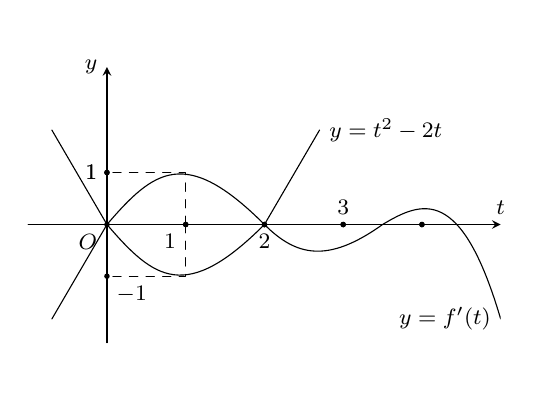
\begin{tikzpicture}[scale=1, font=\footnotesize,line join=round, line cap=round, >=stealth]
	\draw[->] (-1,0)--(5,0) node[above] {$t$};
	\draw[->] (0,-1.5)--(0,2) node[left] {$y$};
    \clip(-1,-2) rectangle (5,2.5);
	\fill (0,0) circle (1pt) node [below left] {$O$};
	\draw (-0.7,-1.2)--(0,0) .. controls (0.6,0.7) and (1,1) .. (2,0)
	(2,0) .. controls (2.4,-0.4) and (2.8,-0.5) .. (3.5,0)
	(3.5,0) .. controls (4,0.3) and (4.5,0.5) .. (5,-1.2) node [left] {$y=f'(t)$};
	\fill (3,0) circle(1pt)node [above] {$3$} (4,0) circle(1pt) (1,0) circle(1pt)
	(2,0) circle (1pt) (0,0.66) circle (1pt) node [left] {$1$};
\draw (-0.7,1.2)--(0,0) .. controls (0.6,-0.7) and (1,-1) .. (2,0)--(2.7,1.2) node [right] {$y=t^2-2t$};
\fill (3,0) circle(1pt) (4,0) circle(1pt) (1,0) circle(1pt) node [below left] {$1$}
(2,0) circle (1pt) (0,0.66) circle (1pt) node [left] {$1$};
	\foreach \x in {2} \fill (\x,0) circle (1pt) node [below] {$\x$};
	%\foreach \x in {-1,1,2} \fill (0,\x) circle (1pt) node [left] {$\x$};
	\draw[dashed] (1,0)|-(0,0.656);
	\draw[dashed] (1,0)|-(0,-0.656);
	\fill (0,-0.656) circle(1pt)node [below right] {$-1$};
\end{tikzpicture}}
\noindent  Xét hàm số $g(t)=f(t)-\dfrac{1}{3} (t-1)^{3}+t-1$	với $t\in [1;3]$.\\
$g'(t)=f'(t)-t^2+2t>0\Leftrightarrow f'(t)>t^2-2t$. Ta vẽ thêm đồ thị $y=t^2-2t$.\\
Từ đồ thị của hàm số $y=f'(t)$ và $y=t^2-2t$ ta thấy $g'(t)=0\Leftrightarrow t=2$ và có bảng xét dấu như sau
\begin{center}
	
\begin{tikzpicture}
		\tkzTabInit[nocadre=false,lgt=1.2,espcl=3,deltacl=0.9]
		{$t$ /0.6,$g'(t)$ /0.6}
		{$1$,$2$,$3$}
		\tkzTabLine{,+,$0$,-,}
	\end{tikzpicture}
\end{center}
Khi đó bảng biến thiên của $g(t)$ như sau

\begin{center}
	
\begin{tikzpicture}
		\tkzTabInit[nocadre=false,lgt=1.2,espcl=3,deltacl=0.9]
		{$t$ /0.6,$g(t)$ /2}
		{$1$,$2$,$3$}
		\tkzTabVar{-/$f(1)$, +/$f(2)+\dfrac{2}{3}$,-/$f(3)-\dfrac{2}{3}$}
	\end{tikzpicture}
\end{center}
Vậy yêu cầu bài toán suy ra $m<f(2)+\dfrac{2}{3}$.}
\end{ex}

\Closesolutionfile{ans}
\begin{indapan}{10}{ans/ans-2-GHK1-30-NguyenDuyHieu-QuangNam-21}
	\end{indapan}
